\documentclass[11pt]{article}
\usepackage[T1]{fontenc}
\usepackage[utf8]{inputenc}
\usepackage[letterpaper]{geometry}

\usepackage{graphicx}
\usepackage{mathpazo}

\usepackage{amsmath}
\usepackage{amsfonts}
\usepackage{bm}
\usepackage{siunitx}
\usepackage{cancel}
\usepackage{float}
\usepackage{empheq}
\usepackage[most]{tcolorbox}

% Sexy yellow highlighted boxed equations!
\newtcbox{\mymath}[1][]{%
	nobeforeafter, math upper, tcbox raise base,
	enhanced, colframe=black!30!black,
	colback=yellow!30, boxrule=1pt,
	#1}

% Hyperlinks with decent looking default colors.
\usepackage{hyperref}
\usepackage{xcolor}
\hypersetup{
	colorlinks,
	linkcolor={red!50!black},
	citecolor={blue!50!black},
	urlcolor={blue!80!black}
}

% For those sexy spaced low small caps from classic-thesis!
\usepackage{microtype}
\usepackage{textcase}
\DeclareRobustCommand{\spacedlowsmallcaps}[1]{%
	\textls[80]{\scshape\MakeTextLowercase{#1}}%
}

% Replaced mathpazo \sum symbol with computer modern's.
\DeclareSymbolFont{cmlargesymbols}{OMX}{cmex}{m}{n}
\let\sumop\relax
\DeclareMathSymbol{\sumop}{\mathop}{cmlargesymbols}{"50}

% Force indent command.
\newcommand{\forceindent}{\leavevmode{\parindent=1em\indent}}

% Math shortcuts.
\newcommand\p[2]{\frac{\partial #1}{\partial #2}}

% fancyhdr header and footer.
\usepackage{fancyhdr}
\pagestyle{fancy} 
\fancyhead{}
\rhead{Ali Ramadhan}
\chead{}
\lhead{12.818: Project 6}
\cfoot{}
\rfoot{\thepage}

\title{\spacedlowsmallcaps{\small 12.818: Introduction to Atmospheric Data and Large-scale Dynamics}\\ \spacedlowsmallcaps{\large Project seven: The Quasi-geostrophic Vorticity Equation}}
\author{\spacedlowsmallcaps{Ali Ramadhan}}
\date{}

\begin{document}
\maketitle

In this project we will study synoptic systems by employing the \emph{quasi-geostrophic vorticity equation}, which can be expressed mathematically in pressure coordinates as
\begin{equation*}
  \frac{D_g}{Dt}(\zeta_g + f) = -f (\nabla \cdot \bm{v}) = f\p{\omega}{p}
  = \frac{f}{\varrho} \p{(\varrho w)}{z}
\end{equation*}
where
\begin{equation*}
  \frac{D_g}{Dt} = \frac{\partial}{\partial t} + \bm{v}_g \cdot \nabla
\end{equation*}
is the geostrophic derivative operator, $\zeta_g + f$ is the absolute vorticity, $f$ is the planetary vorticity, $\zeta_g$ is the geostrophic relative vorticity evaluated on an isobaric surface, $\omega$ is the vertical velocity in pressure coordinates, $w$ is the vertical velocity in height coordinates, $\bm{v}$ is the wind velocity field, and $\bm{u}_g$ is the geostrophic wind velocity field.

Flows in \emph{quasi-geostrophic motion} have the Coriolis force and pressure  gradient forces \emph{almost} balancing each other, with interia providing the residual effect, as opposed to geostrophic balance where the Coriolis and pressure gradient forces are exactly in balance.

The quasi-geostrophic equation exhibits some useful properties. One is that it states that the sum of the relative, planetary, and stretching vorticities must be conserved following geostrophic motions. Another is that it allows for the determination of the geostrophic wind velocity and temperature fields from knowledge of the geopotential height only. Furthermore, if the time evolution of the geopotential height field is also known, vertical motions in the atmosphere may be inferred.

Note that the \emph{absolute vorticity} $\bm{\omega}$ is the curl of the absolute velocity, $\bm{\omega} = \nabla \cdot \bm{u}_a$, while the \emph{relative vorticity} $\bm{\omega}$ is the curl of the relative velocity, $\bm{\omega} = \nabla \cdot \bm{u}$. Furthermore, in meteorology, we are generally interested in the vertical components of the absolute vorticity, denoted $\eta$, and the vertical component of the relative vorticity, denoted $\zeta$, where $\eta = \hat{\bm{z}} \cdot \bm{\omega}_a$ and $\zeta = \hat{\bm{z}} \cdot \bm{\omega}$. The difference between the absolute and relative vorticity is called the \emph{planetary vorticity}, and denoted $f$ where $f = \hat{\bm{z}} \cdot (\nabla \times \bm{u}_e) = 2\Omega\sin\phi$ which happens to be the Coriolis parameter and thus $\eta = \zeta + f$.

Note that positive vorticity is associated with low pressure systems or cyclonic storms in the Northerm Hemisphere, while negative vorticity is associated with high pressure systems. In the Southern Hemisphere, negative vorticity is associated with cyclonic storms.

% Also note that the local rate of change of geostrophic vorticity is determined by the sum of two terms; the advection of the absolute vorticity by the geostrophic wind, and the the stretching or shrinking of fluid columns via a  divergence.

\section{Quasi-geostrophic scaling}
In this section we will estimate the scales associated with a synoptic system and compare them to the predicted quasi-geostrophic scaling. To identify synoptic systems we plot the mean sea level pressure over North America on November 2, 2017 (0Z) in figure \ref{fig:pmsl_nam}. Unfortunately the weather looks relatively boring around Boston, MA, however, there is a low pressure system to the west over the central United States centered over the states of Colorado, Nebraska, and Kansas, as well as a high pressure system to the east over the Northern Atlantic Ocean.

\begin{figure}[h!]
	\centering
	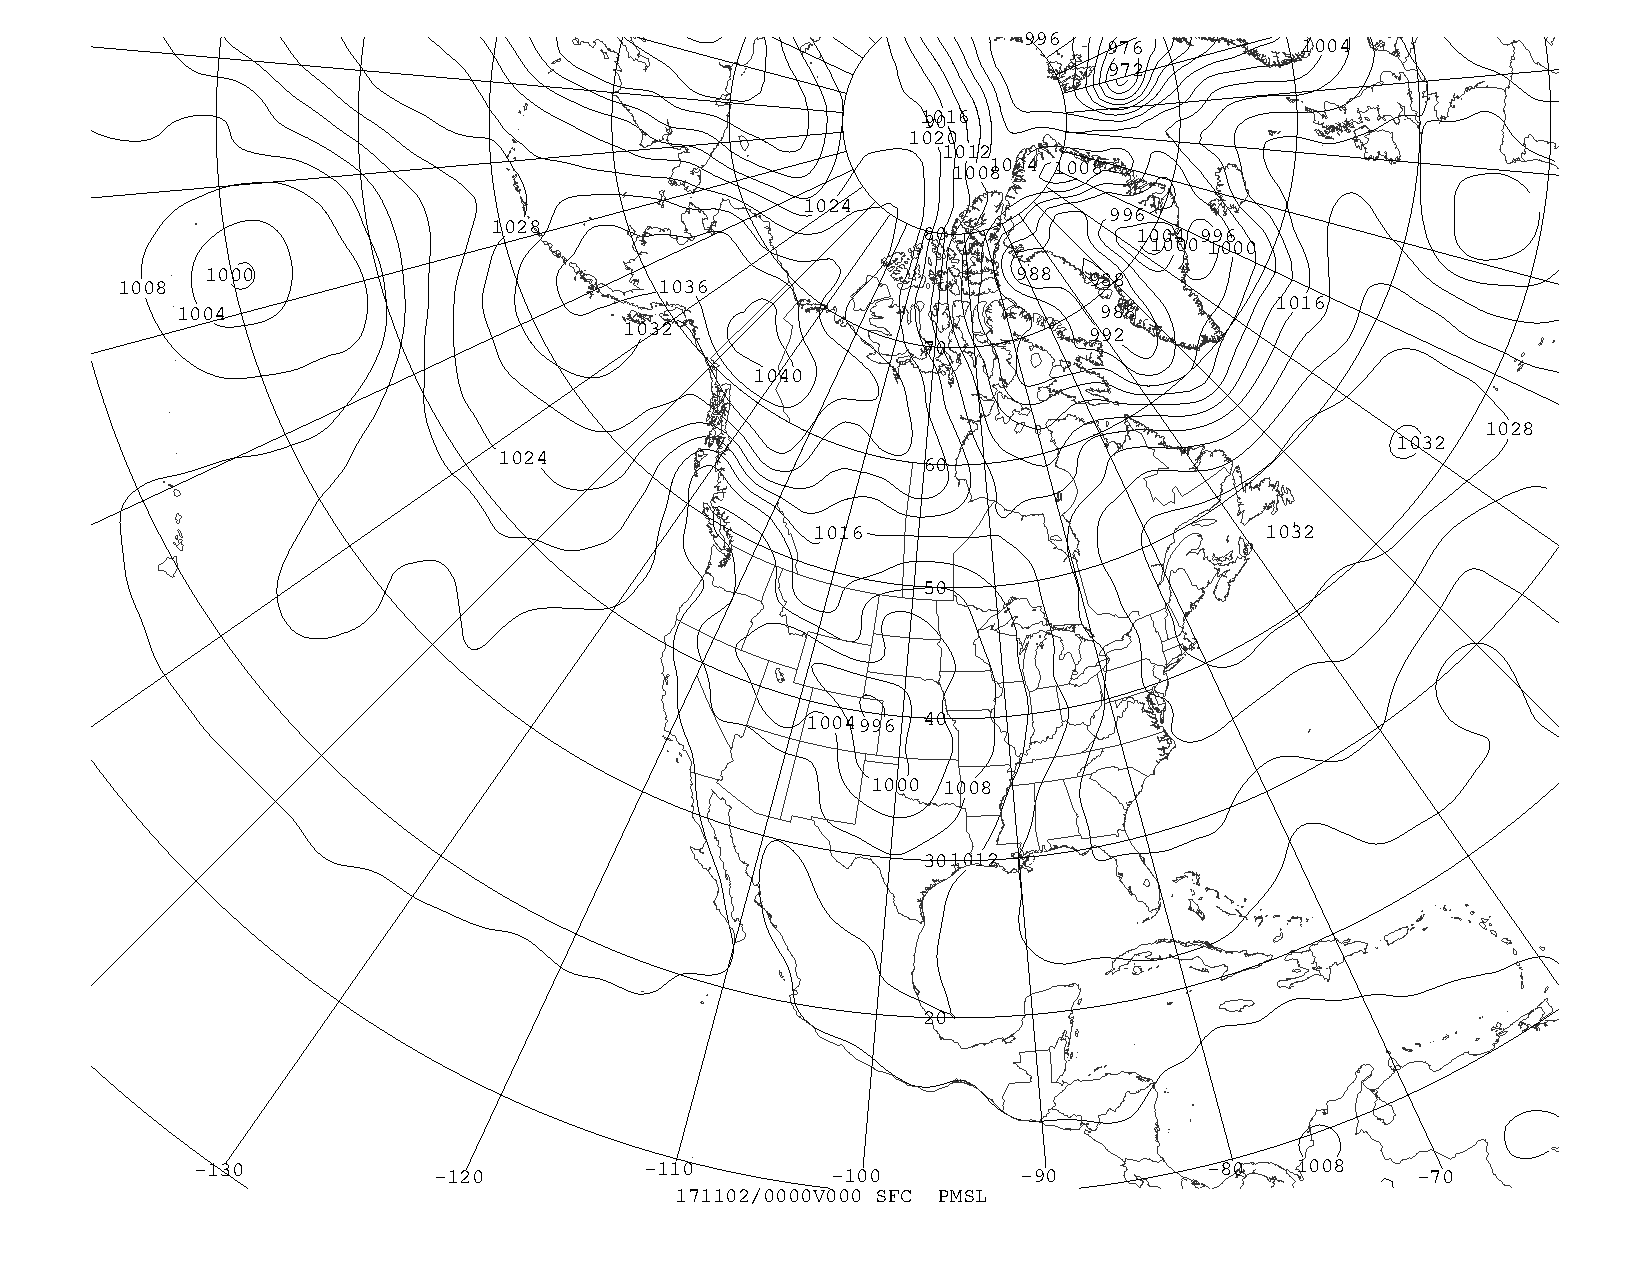
\includegraphics[width=\textwidth]{pmsl_nam}
	\caption{Contour plot of the mean sea level pressure over North America on November 2, 2017 (0Z).}
	\label{fig:pmsl_nam}
\end{figure}

Figure \ref{fig:thta_normwnd_mer_xsec} shows a meridional cross-section of the potential temperature (K) and observed wind velocity (normal to the cross-section) through Boston, MA from \SI{25}{\degree N} to \SI{70}{\degree N}, while figure \ref{fig:thta_normwnd_zon_xsec} shows a zonal cross-section from \SI{120}{\degree W} to \SI{20}{\degree E}, both on November 2, 2017 (0Z). We will be more interested in the zonal cross-section (figure \ref{fig:thta_normwnd_zon_xsec}) as it passes through the low and high pressure systems we identified in figure \ref{fig:pmsl_nam}. In particular we will focus on the low-pressure system.

\begin{figure}[h!]
  \centering
  % trim={0 0 3.5cm 0}, clip,
  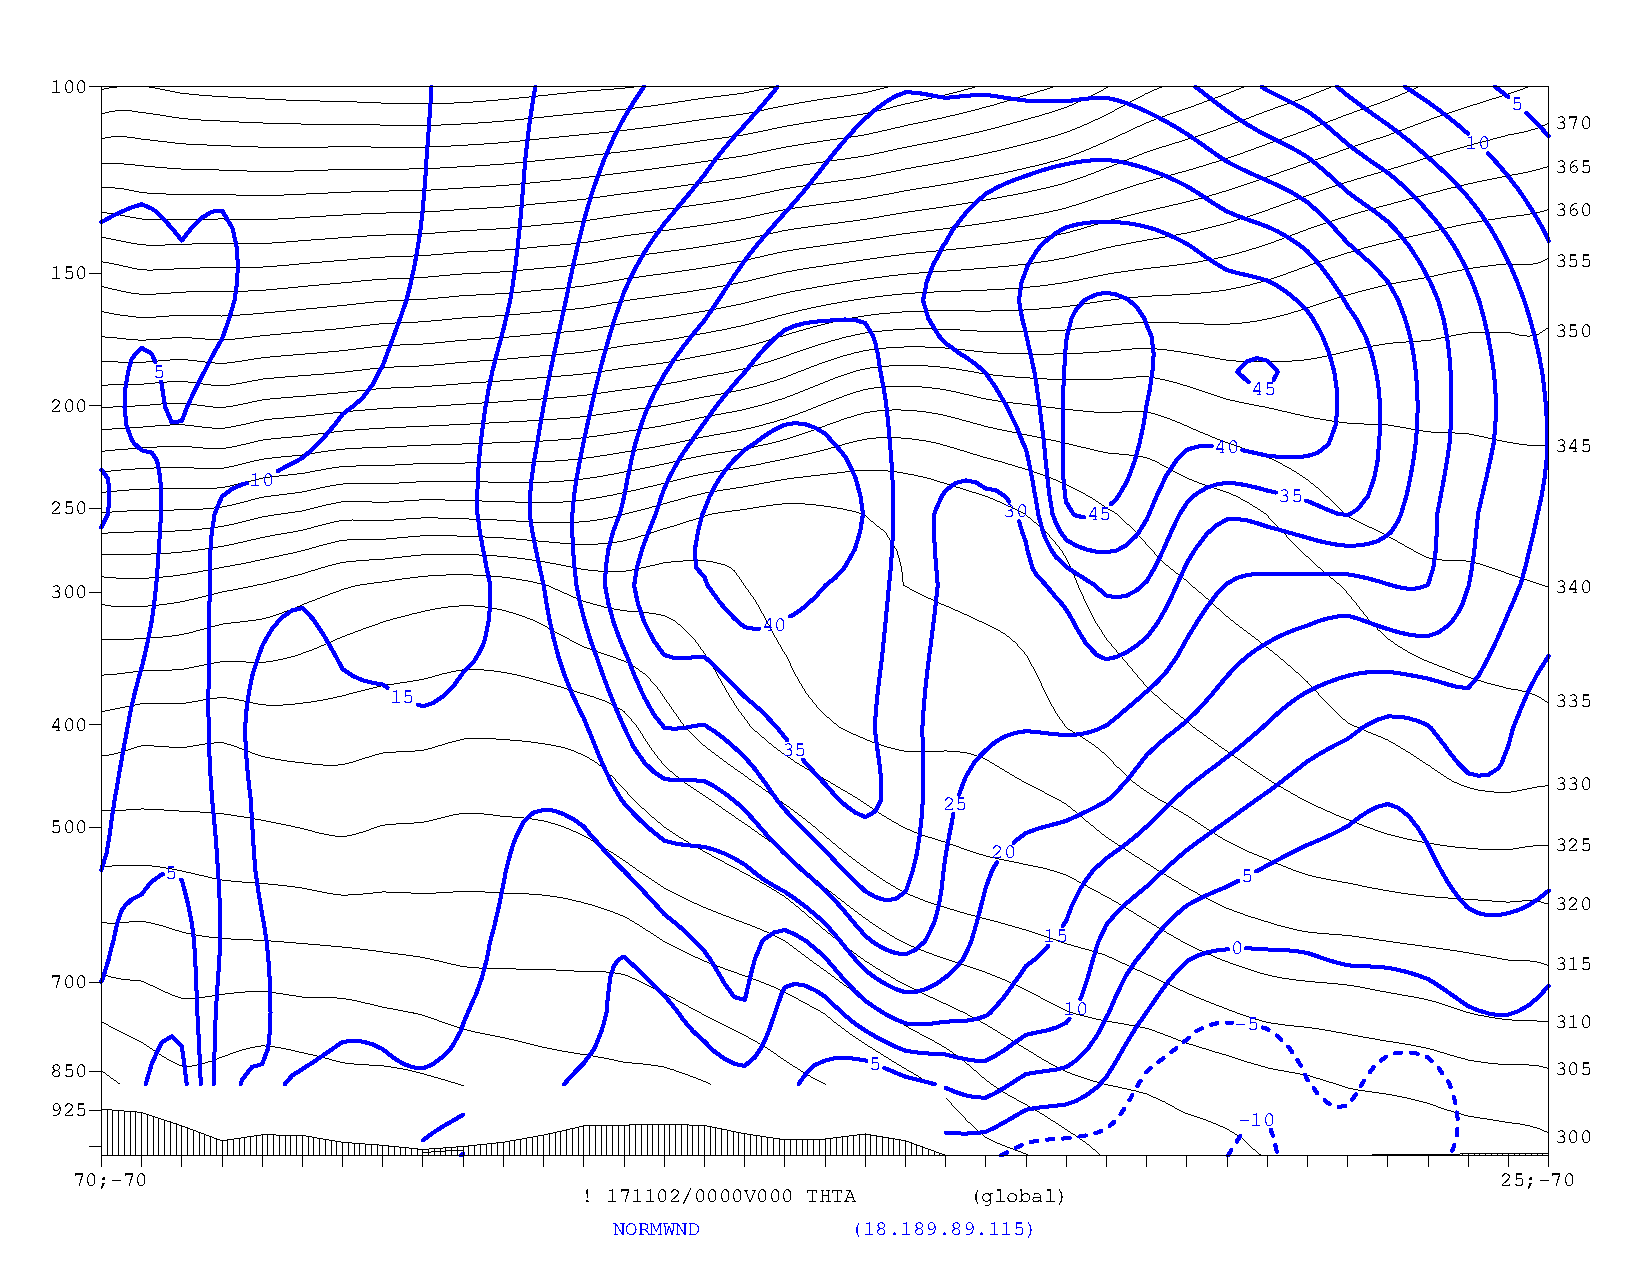
\includegraphics[width=\textwidth]{thta_normwnd_70W_25-70N}
  \caption{Meridional cross-section of the potential temperature (K) and observed wind velocity (normal to the cross-section) from \SI{25}{\degree N} to \SI{70}{\degree N} along the \SI{70}{\degree W} meridian (chosen to pass through Boston, MA) on November 2, 2017 (0Z).}
  \label{fig:thta_normwnd_mer_xsec}
\end{figure}

\begin{figure}[h!]
  \centering
  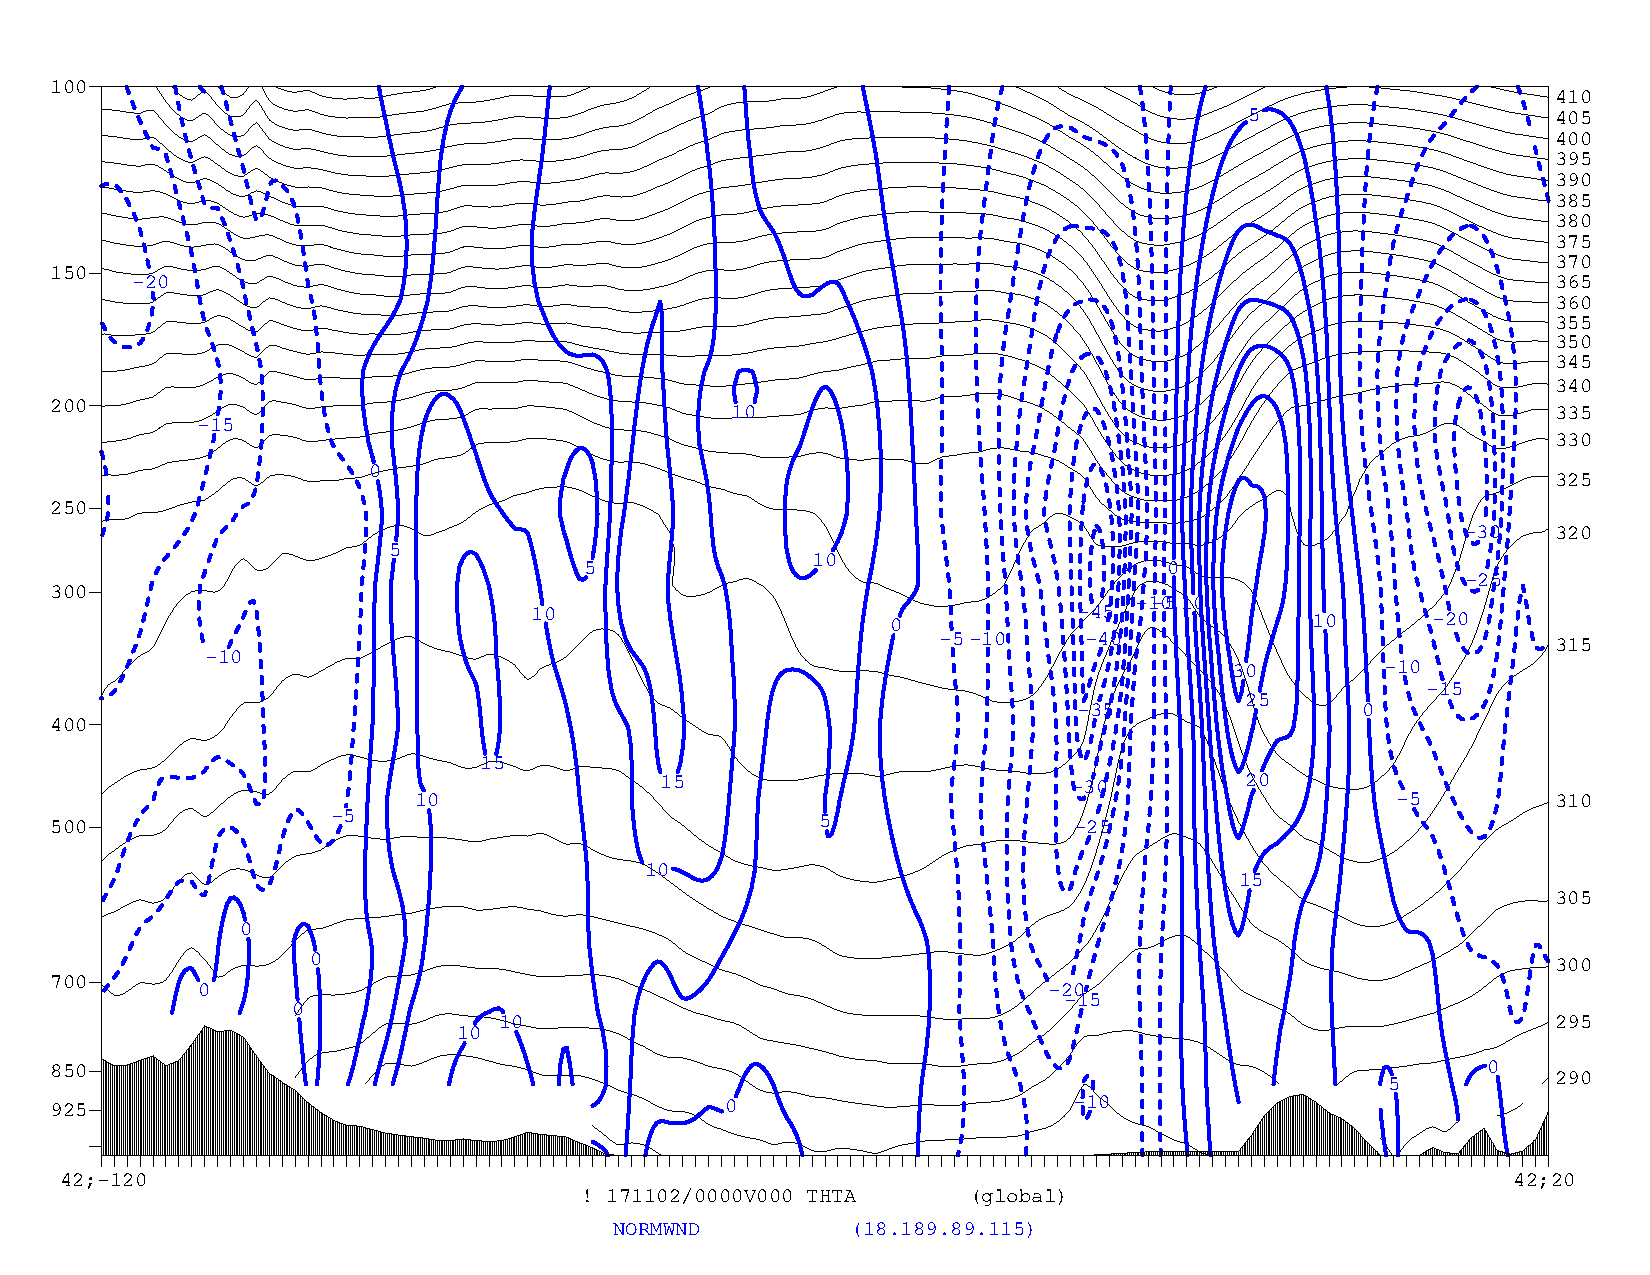
\includegraphics[width=\textwidth]{thta_normwnd_42N_120W-20E}
  \caption{Zonal cross-section of the potential temperature (K) and observed wind velocity (normal to the cross-section) from \SI{120}{\degree W} to \SI{20}{\degree E} along the \SI{42}{\degree N} meridian (chosen to pass through Boston, MA) on November 2, 2017 (0Z).}
  \label{fig:thta_normwnd_zon_xsec}
\end{figure}

We can estimate the troposhperic scale height $\displaystyle H = \frac{R T_0}{g}$ where $T_0$ represents a mean tropospheric temperature in the region of the system. By inspection of the potential temperature contours over the low-pressure system in figure \ref{fig:thta_normwnd_zon_xsec} we see that $T_0 = \SI{290}{\K}$ is a reasonable estimate of the surface temperature as potential temperature and air temperature coincide at mean sea level pressure. The actual air temperature may be higher due to the low-pressure system being near the Rocky Mountains which are significantly above sea level. Using $R = \SI{287.058}{\J/\kg.\K}$ this gives us a tropospheric scale height of $H = \SI{8.5}{\km}$ which seems reasonable for the mid-latitudes.

We can estimate the buoyancy frequency $\displaystyle N^2 = \frac{g}{\vartheta_0} \p{\vartheta}{z}$ where $\vartheta_0$ is a reference mean potential temperature.

\section{The Quasi-geostrophic vorticity equation}

\begin{figure}[h!]
	\centering
	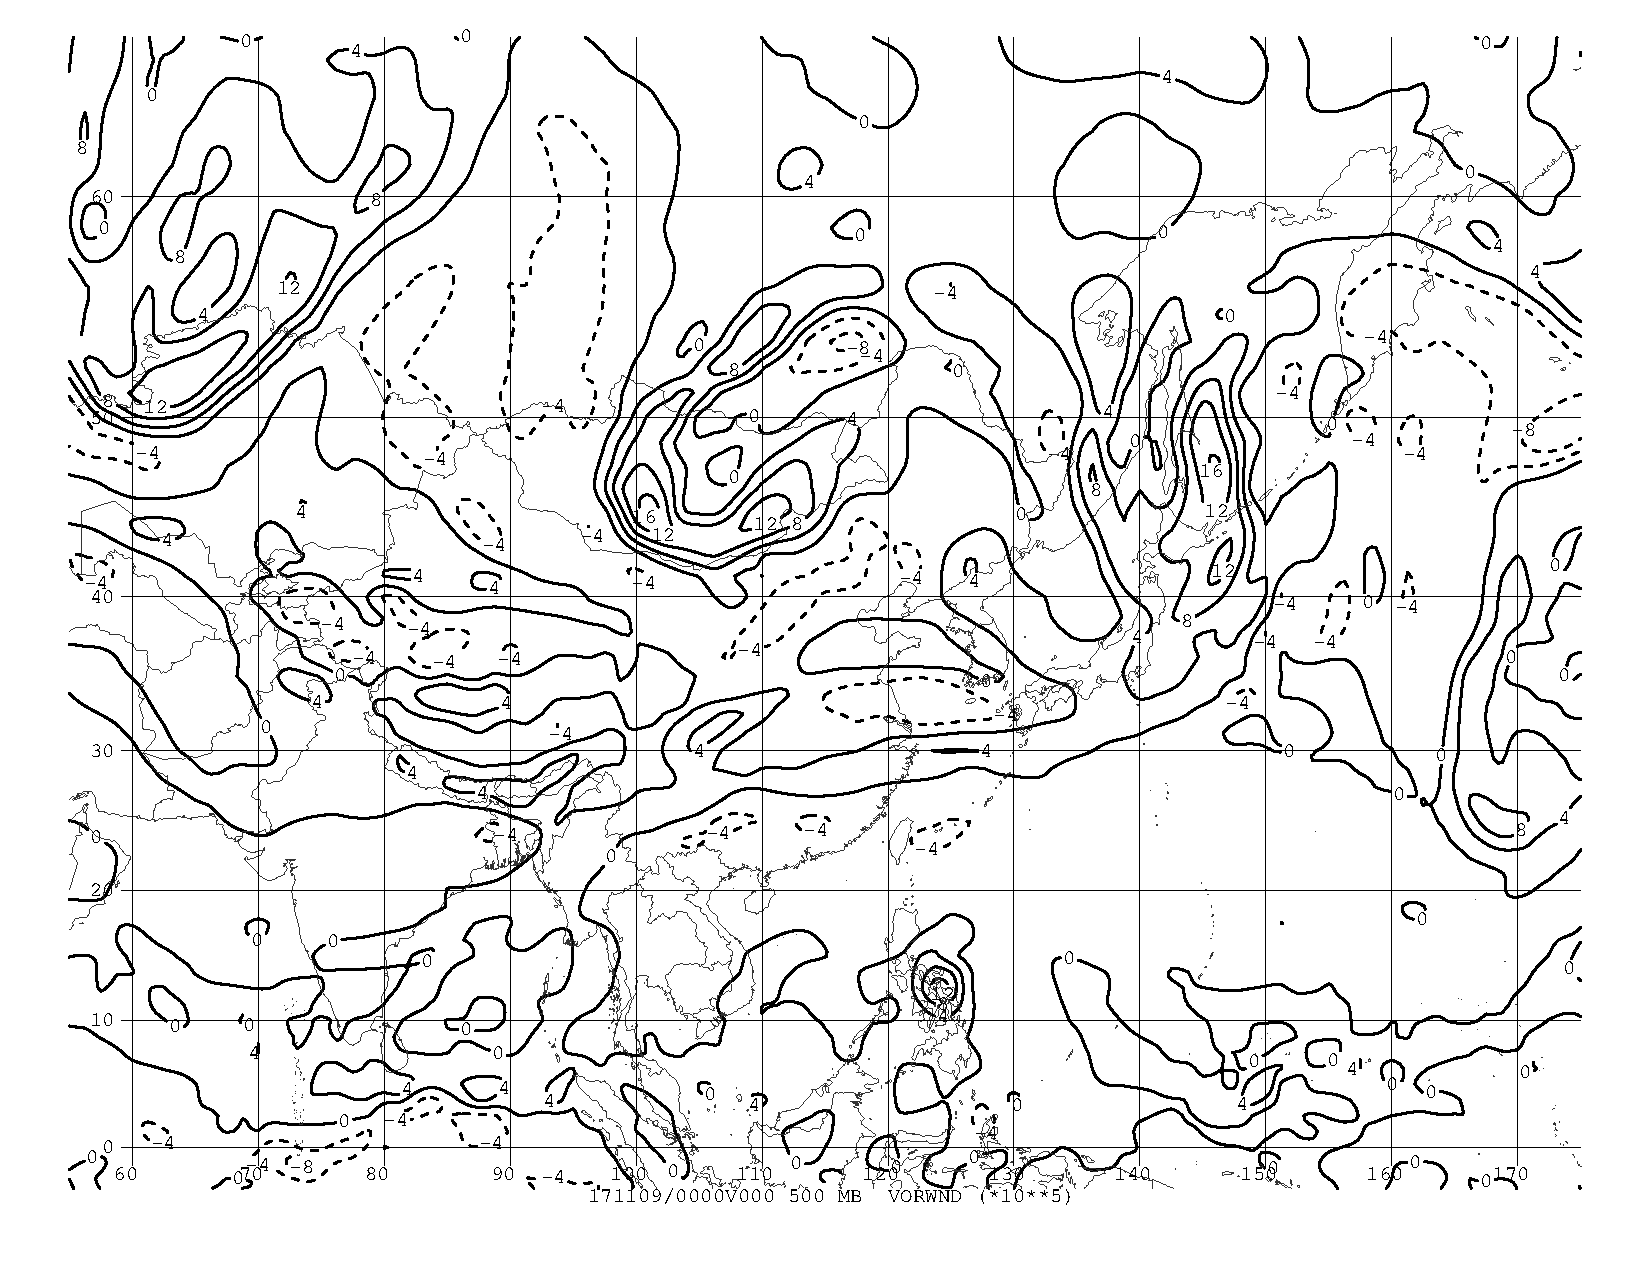
\includegraphics[width=\textwidth]{vorwnd_obs_500hPa_China}
	\caption{Contour plot of the vorticity ($\times 10^5$) field calculated from the observed wind velocity field at \SI{500}{\hecto\Pa} over Eastern Asia on November 9, 2017 (0Z).}
	\label{fig:vorwnd_obs_500hPa_China}
\end{figure}

\begin{figure}[h!]
	\centering
	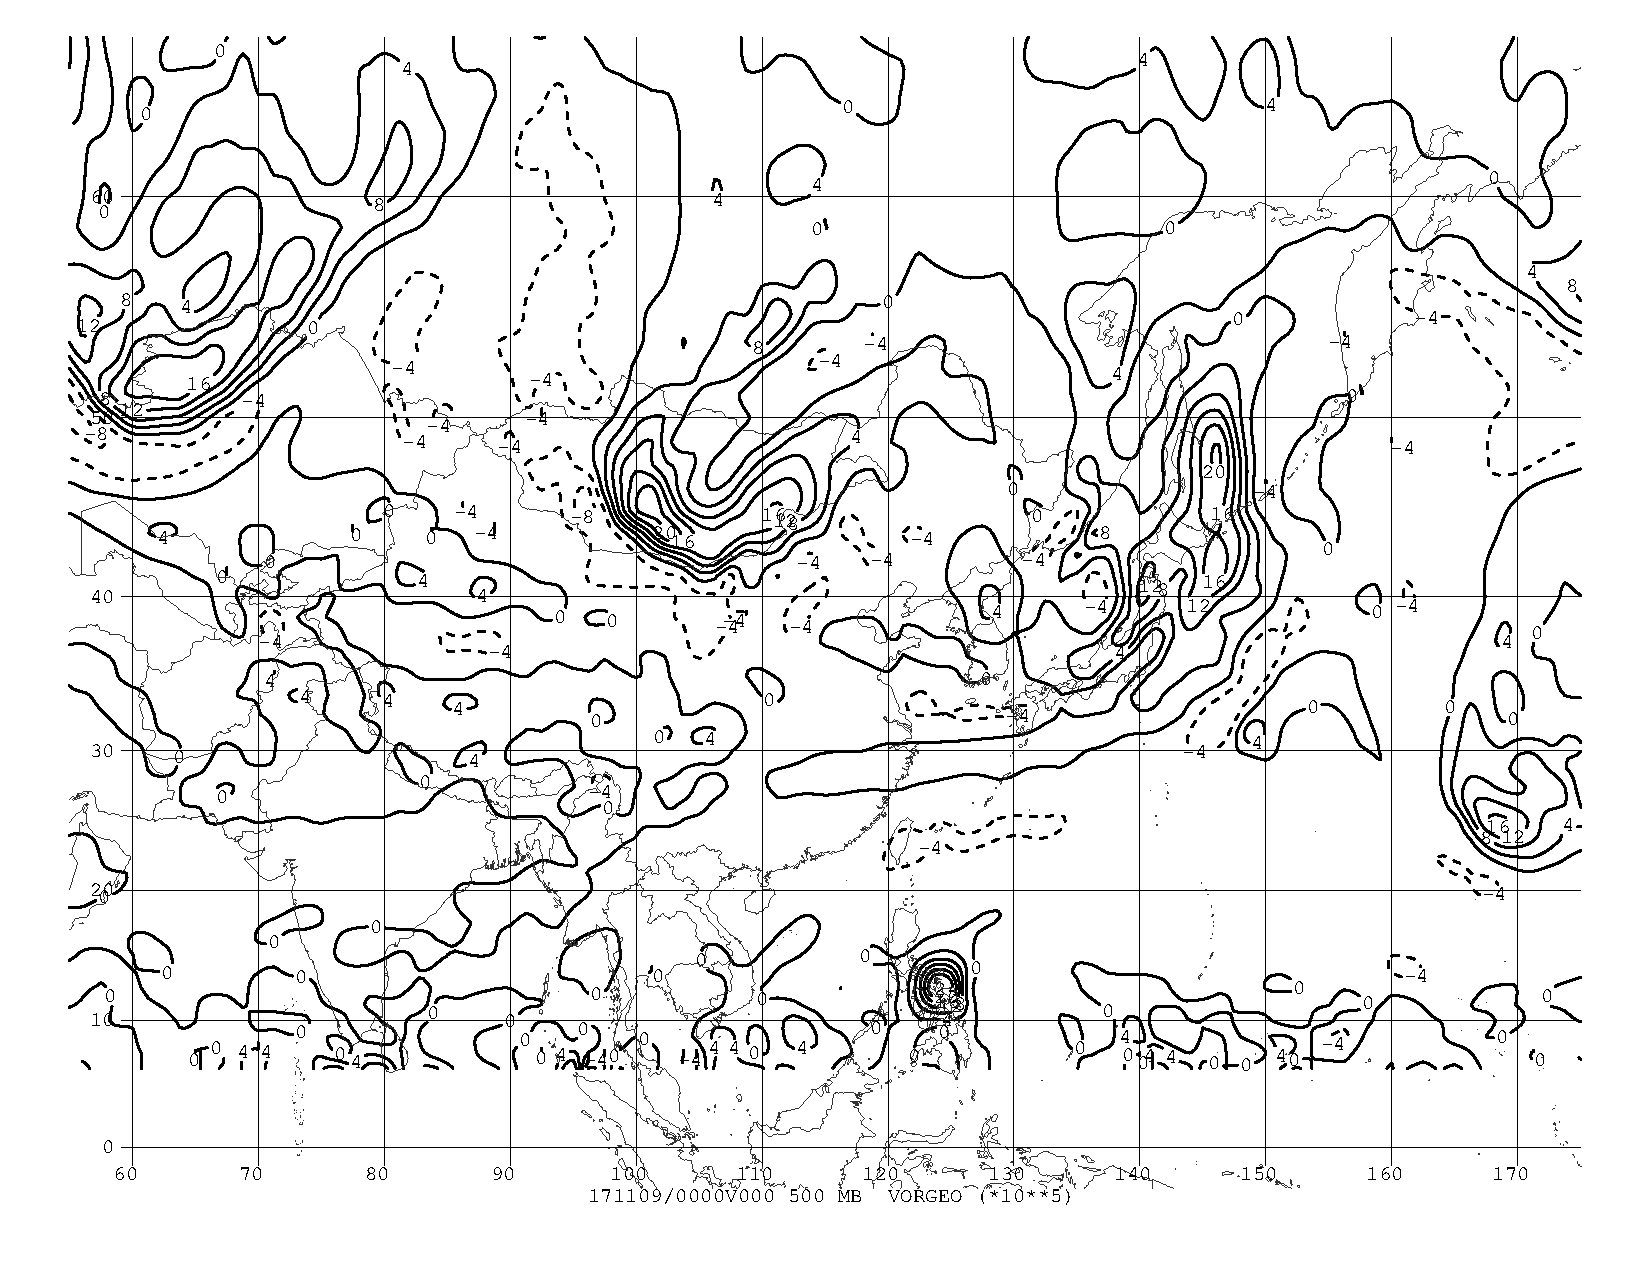
\includegraphics[width=\textwidth]{vorgeo_500hPa_China}
	\caption{Contour plot of the geostrophic vorticity ($\times 10^5$) field (that is, calculated from the geostrophic wind velocity field) at \SI{500}{\hecto\Pa} over Eastern Asia on November 9, 2017 (0Z).}
	\label{fig:vorgeo_obs_500hPa_China}
\end{figure}

\begin{figure}[h!]
	\centering
	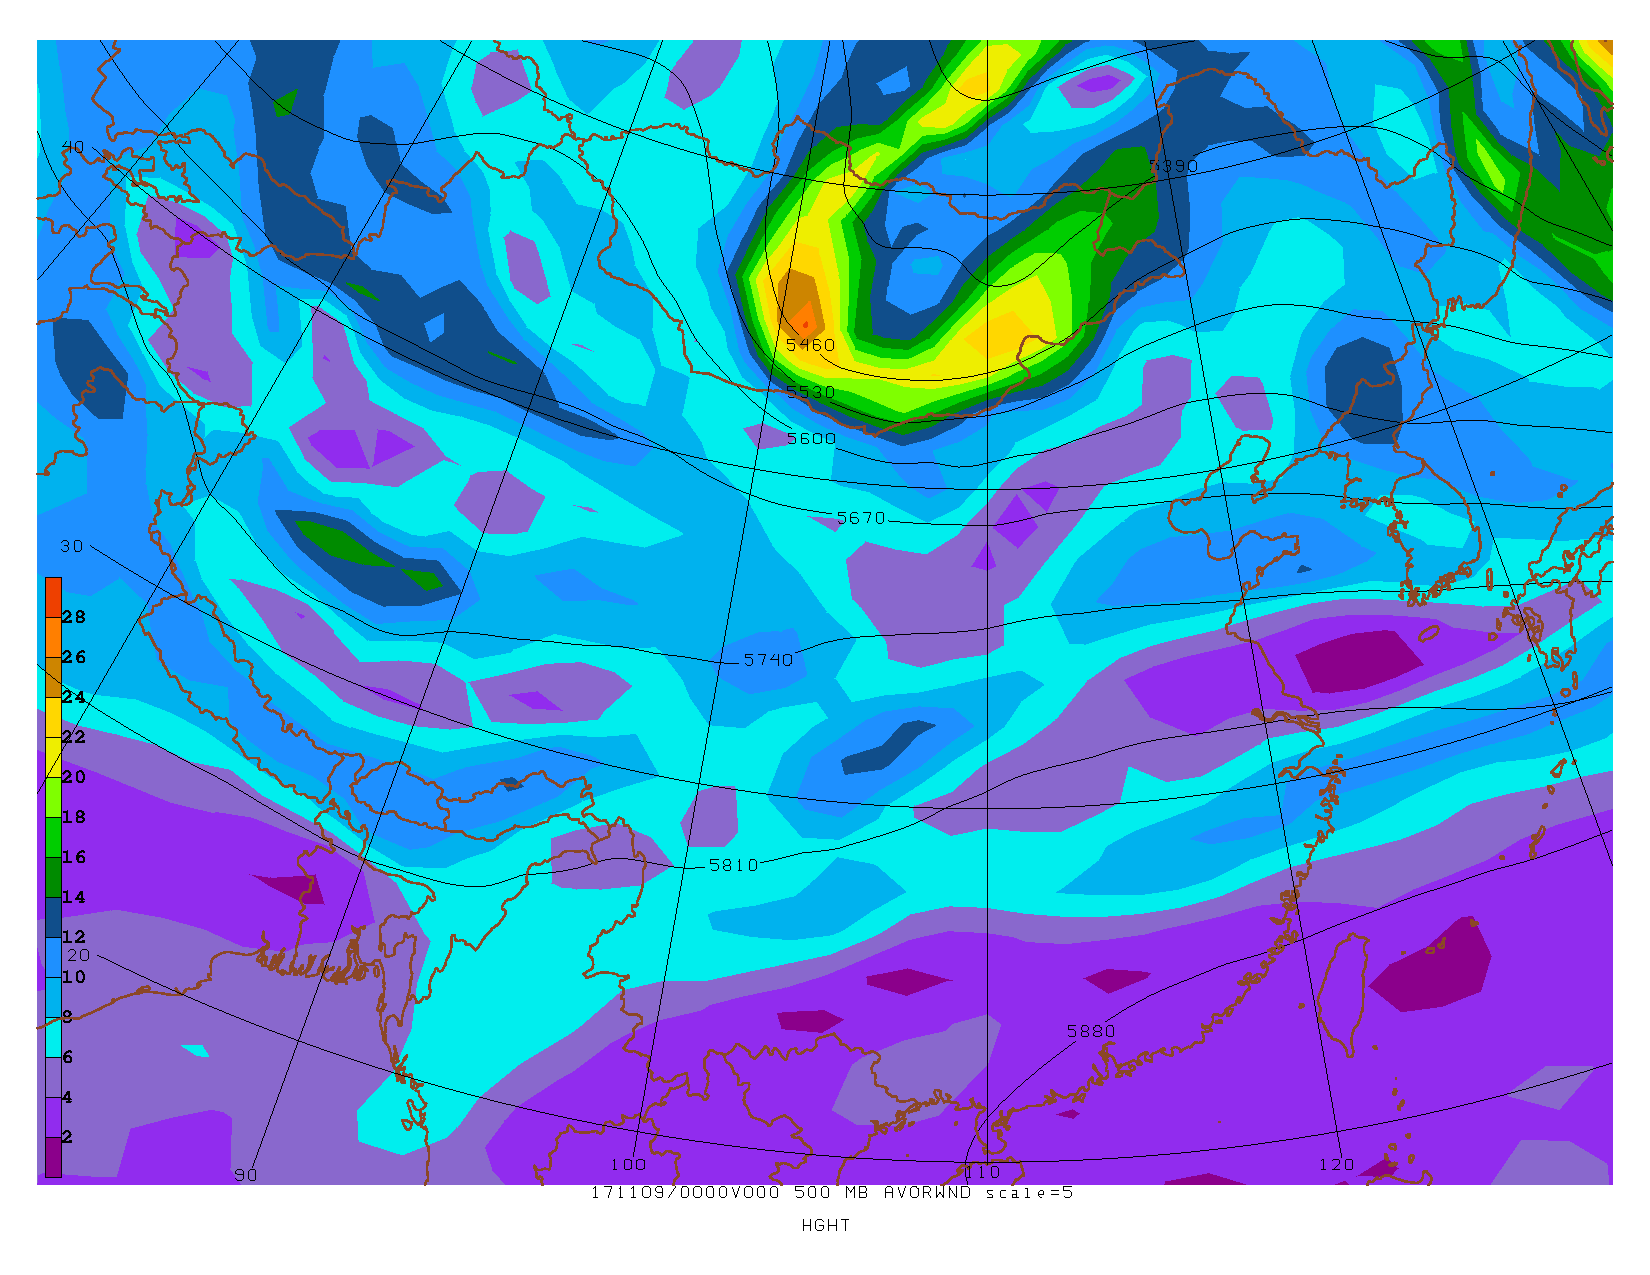
\includegraphics[width=\textwidth]{avorwnd_500hPa_China}
	\caption{Contour plot of the absolute vorticity $\zeta_g + f$ ($\times 10^5$) and geopotential height field at \SI{500}{\hecto\Pa} over Eastern Asia on November 9, 2017 (0Z).}
	\label{fig:avorwnd_500hPa_China}
\end{figure}

\begin{figure}[h!]
	\centering
	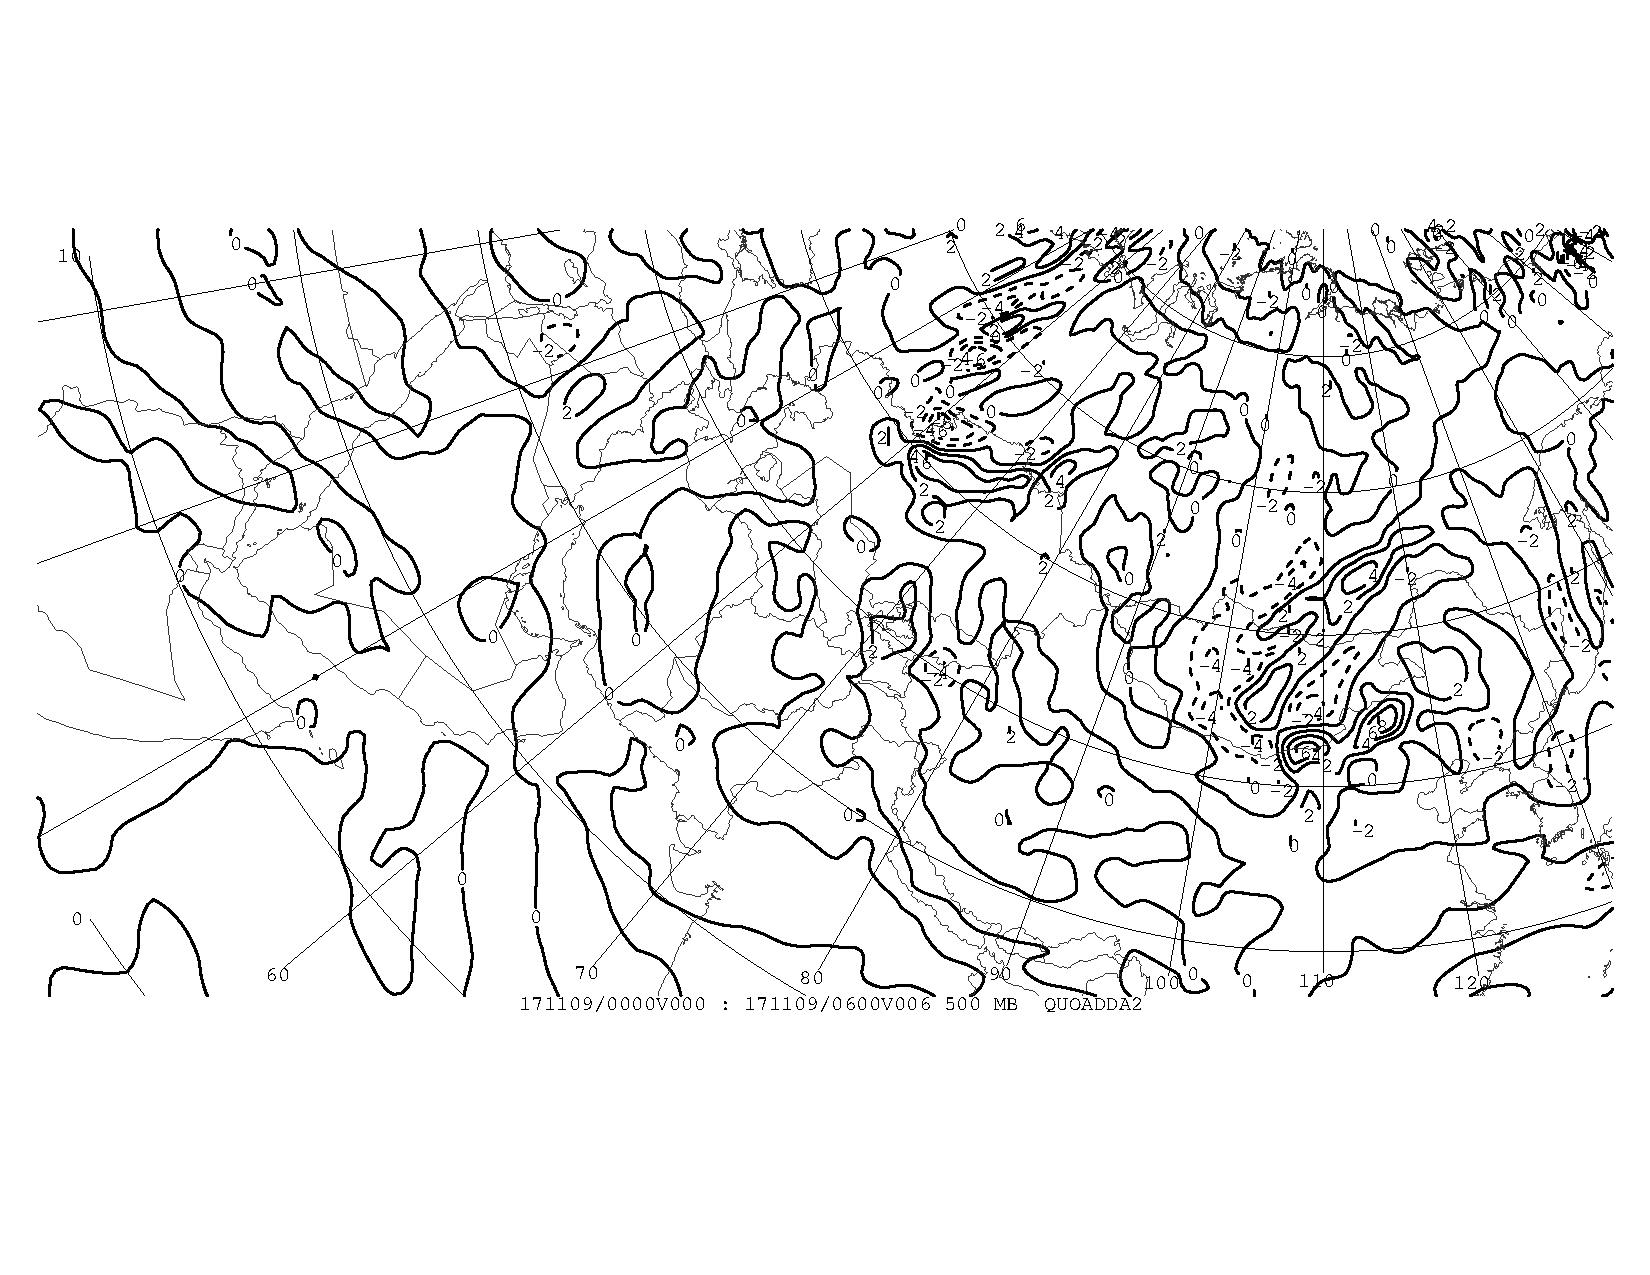
\includegraphics[width=\textwidth]{horizontal_advection_avor_500hPa_China}
	\caption{Contour plot of the horizontal advection of absolute vorticity $\bm{u}_g \cdot \nabla(\zeta_g + f)$ ($\times 10^5$) and geopotential height field at \SI{500}{\hecto\Pa} over Eastern Asia on November 9, 2017 (0Z).}
	\label{fig:horizontal_advection_avor_500hPa_China}
\end{figure}

\begin{figure}[h!]
	\centering
	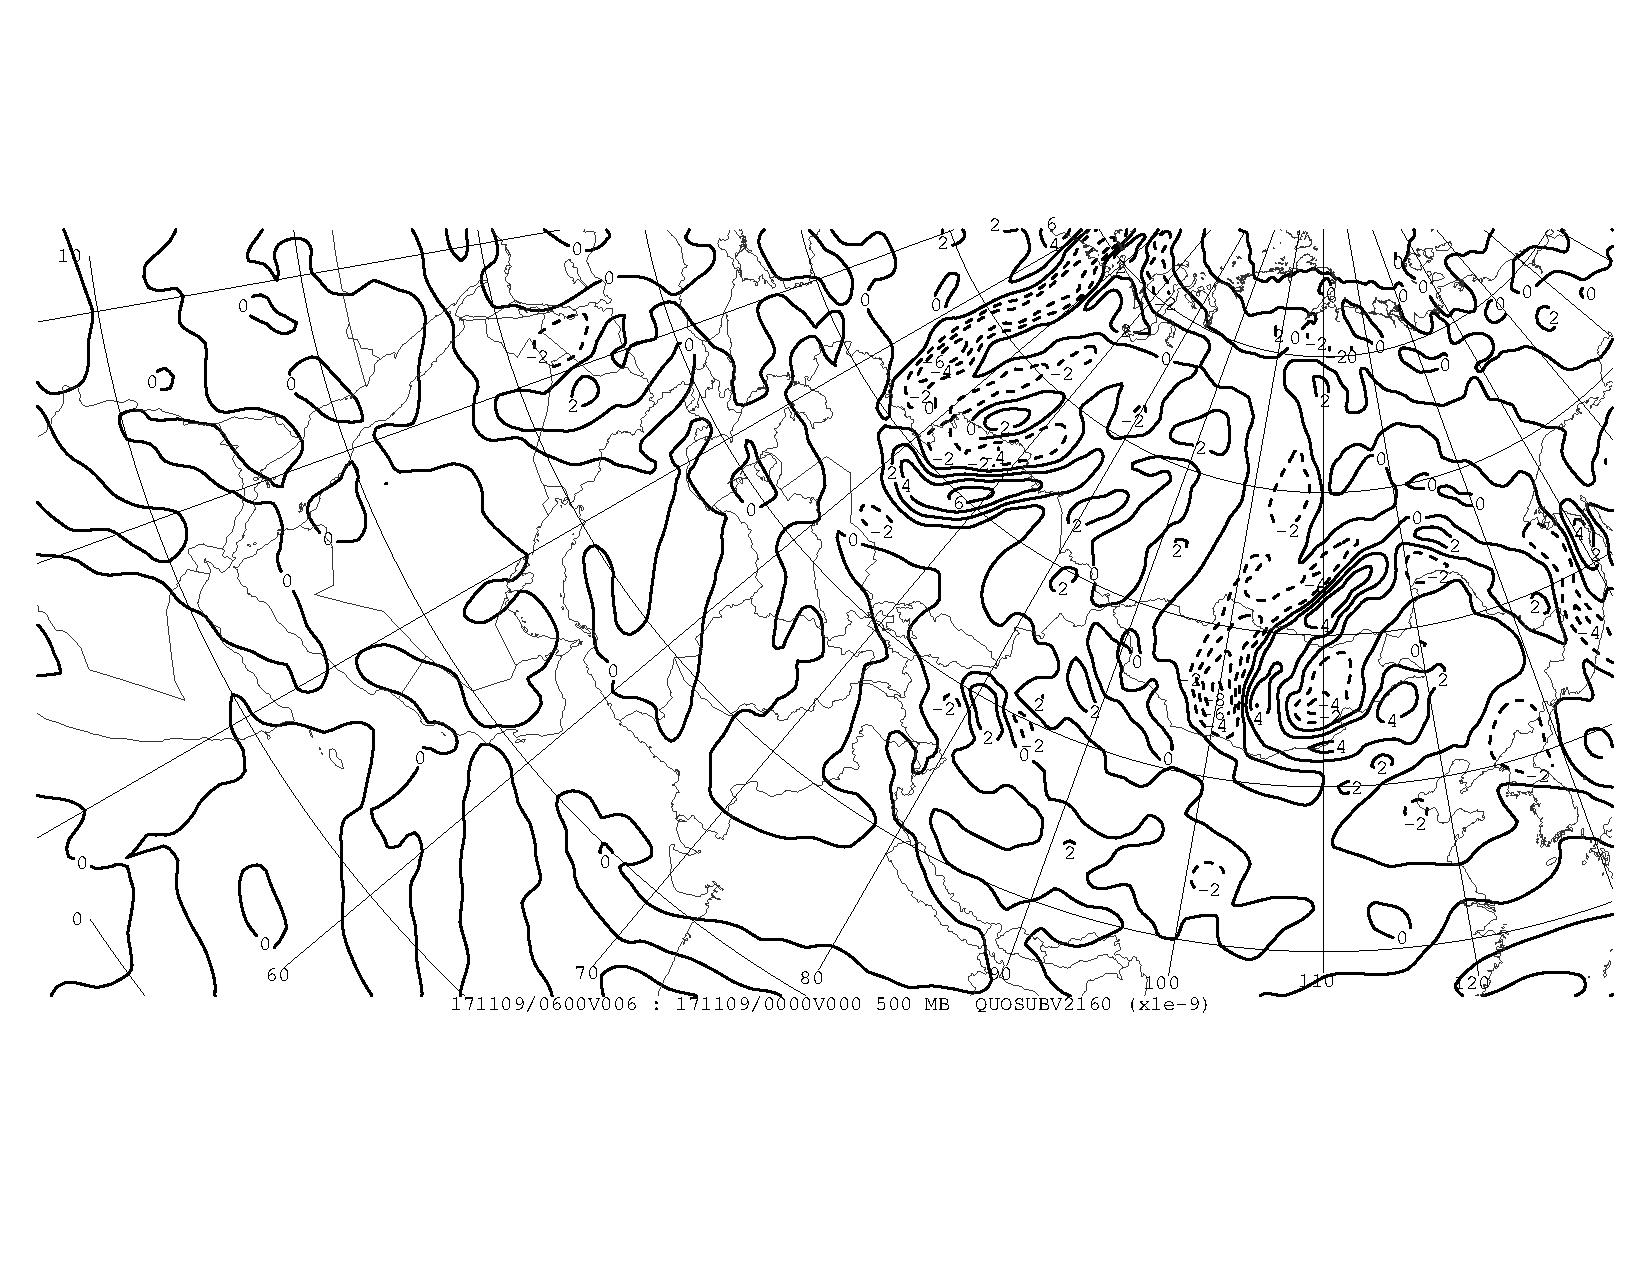
\includegraphics[width=\textwidth]{dvordt_500hPa_China}
	\caption{Contour plot of the rate of change of relative vorticity $\partial\zeta/\partial t$ ($\times 10^9$) and geopotential height field at \SI{500}{\hecto\Pa} over Eastern Asia on November 9, 2017 (0Z).}
	\label{fig:dvordt_500hPa_China}
\end{figure}


\section{The Brunt--Väisälä frequency}



\end{document}